\begin{tikzpicture}[
        font=\small,
        thick,
        node distance=0mm,
        every node/.style={inner sep=0, outer sep=0},
        top label/.style={anchor=north west, xshift=0.3cm, yshift=-0.3cm},
        bottom label/.style={anchor=south west, xshift=0.3cm, yshift=0.3cm},
        title/.style={anchor=text, yshift=2.5mm}
    ]

    \node (h_orig) {
            
\includegraphics[width=\figurewidth,
                             trim=0 100 0 50,
                             clip]
                            {images/data3/H_orig_rdoryl.png}
    };
    \node[top label] at (h_orig.north west) {Original};
    \node[anchor=east, draw=black, inner sep=0.05mm] (cmap) at ($(h_orig.east) + (-1cm, 0)$) {
        \rotatebox{-90}{%
        
\includegraphics[width=2.5cm,height=0.25cm]{figures/rdoryl.png}%
        }%
    };
    \node[anchor=north west, xshift=1mm] at (cmap.north east) {max};
    \node[anchor=south west, xshift=1mm] at (cmap.south east) {min};

    \node[title] at (h_orig.north west) {
        \textsc{\normalsize Syngas II: $\text{H}$}
    };

    \node[anchor=north west, at={($(h_orig.south west) + (0, -2mm)$)}] (h_lin) {
            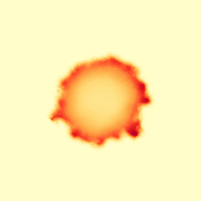
\includegraphics[width=0.33333333\figurewidth-1.3333333mm,
                             trim=30 100 30 30,
                             clip,
                             ]
                            {images/data3/H_lin_36_rdoryl.png}
    };
    \node[top label] at (h_lin.north west) {linear interpolation};

    \node[anchor=north, at={($(h_orig.south) + (0, -2mm)$)}] (h_knn) {
            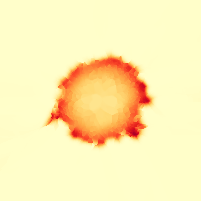
\includegraphics[width=0.33333333\figurewidth-1.3333333mm,
                             trim=30 100 30 30,
                             clip]
                            {images/data3/H_knn_36_rdoryl.png}
    };
    \node[top label] at (h_knn.north west) {k{\otherscshape{ann}} interpolation};

    \node[anchor=north east, at={($(h_orig.south east) + (0, -2mm)$)}] (h_down) {
            
\includegraphics[width=0.33333333\figurewidth-1.3333333mm,
                             trim=30 100 30 30,
                             clip]
                            {images/data3/H_down_36_rdoryl.png}
    };
    \node[top label] at (h_down.north west) {downsampling};

    \node[anchor=north, at={(h_lin.south)}] (h_diff_lin) {
            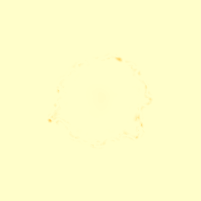
\includegraphics[width=0.33333333\figurewidth-1.3333333mm,
                             trim=30 30 30 100,
                             clip]
                            {images/data3/H_diff_lin_36_rdoryl.png}
    };
    \node[bottom label] at (h_diff_lin.south west) {
        $E^{\text{H}}_{\textnormal{reconst}}$
    };
    \draw[dashed] (h_lin.south west) -- (h_lin.south east);

    \node[anchor=north, at={(h_knn.south)}] (h_diff_knn) {
            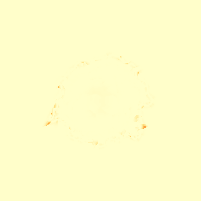
\includegraphics[width=0.33333333\figurewidth-1.3333333mm,
                             trim=30 30 30 100,
                             clip]
                            {images/data3/H_diff_knn_36_rdoryl.png}
    };
    \node[bottom label] at (h_diff_knn.south west) {
        $E^{\text{H}}_{\textnormal{reconst}}$
    };
    \draw[dashed] (h_knn.south west) -- (h_knn.south east);

    \node[anchor=north, at={(h_down.south)}] (h_diff_down) {
            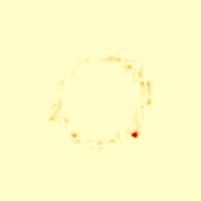
\includegraphics[width=0.33333333\figurewidth-1.3333333mm,
                             trim=30 30 30 100,
                             clip]
                            {images/data3/H_diff_down_36_rdoryl.png}
    };
    \node[bottom label] at (h_diff_down.south west) {
        $E^{\text{H}}_{\textnormal{reconst}}$
    };
    \draw[dashed] (h_down.south west) -- (h_down.south east);



    \node[anchor=north, at={($(h_diff_lin.south) + (0, -1cm)$)}] (o2_orig) {
        
\includegraphics[width=0.33333333\figurewidth-1.3333333mm,
                         trim=105 25 15 95,
                         clip]
                        {images/O2_orig_rdoryl.png}
    };
    \node[top label] at (o2_orig.north west) {Original};

    \node[title] at (o2_orig.north west) {
        \textsc{\normalsize Syngas I: ${\text{O}_2}$}
    };

    \node[anchor=north, at={($(h_diff_knn.south) + (0, -1cm)$)}] (o2_1) {
        
\includegraphics[width=0.33333333\figurewidth-1.3333333mm,
                         trim=105 25 15 95,
                         clip]
                        {images/O2_lin_1_rdoryl.png}
    };
    \node[top label] at (o2_1.north west) {$q=1,\,c=7.6$};

    \node[anchor=north, at={($(h_diff_down.south) + (0, -1cm)$)}] (o2_12) {
        
\includegraphics[width=0.33333333\figurewidth-1.3333333mm,
                         trim=105 25 15 95,
                         clip]
                        {images/O2_lin_12_rdoryl.png}
    };
    \node[top label] at (o2_12.north west) {$q=11.5,\,c=49$};

    \node[anchor=north, at={($(o2_orig.south) + (0, -2mm)$)}] (o2_23) {
        
\includegraphics[width=0.33333333\figurewidth-1.3333333mm,
                         trim=105 25 15 95,
                         clip]
                        {images/O2_lin_23_rdoryl.png}
    };
    \node[top label] at (o2_23.north west) {$q=23.3,\,c=101$};

    \node[anchor=north, at={($(o2_1.south) + (0, -2mm)$)}] (o2_58) {
        
\includegraphics[width=0.33333333\figurewidth-1.3333333mm,
                         trim=105 25 15 95,
                         clip]
                        {images/O2_lin_58_rdoryl.png}
    };
    \node[top label] at (o2_58.north west) {$q=58,\,c=253$};

    \node[anchor=north, at={($(o2_12.south) + (0, -2mm)$)}] (o2_240) {
        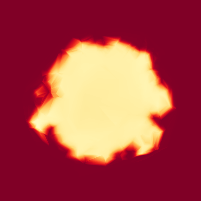
\includegraphics[width=0.33333333\figurewidth-1.3333333mm,
                         trim=105 25 15 95,
                         clip]
                        {images/O2_lin_240_rdoryl.png}
    };
    \node[top label] at (o2_240.north west) {$q=240,\,c=1037$};

\end{tikzpicture}